\documentclass[9pt]{beamer}

\usepackage{booktabs}
\usepackage{geometry}
\usepackage{enumitem}

\usetheme{Copenhagen}

\title{Knowledge Grounding in Retrieval-Augmented LMs \\ Quick Update}
\author{Martin Fixman et. al}
\institute{City, University of London}
\date{6 September 2024}

\begin{document}

\begin{frame}
	\titlepage{}
\end{frame}

\section{Reading List}
\begin{frame}{Reading List}
	\begin{large}
		``Characterizing Mechanisms for Factual Recall in Language Models''
	\end{large} \\
	Yu et. al \\
	\textit{\scriptsize Thanks Chenxi}

	\vfill{}

	\begin{center}
		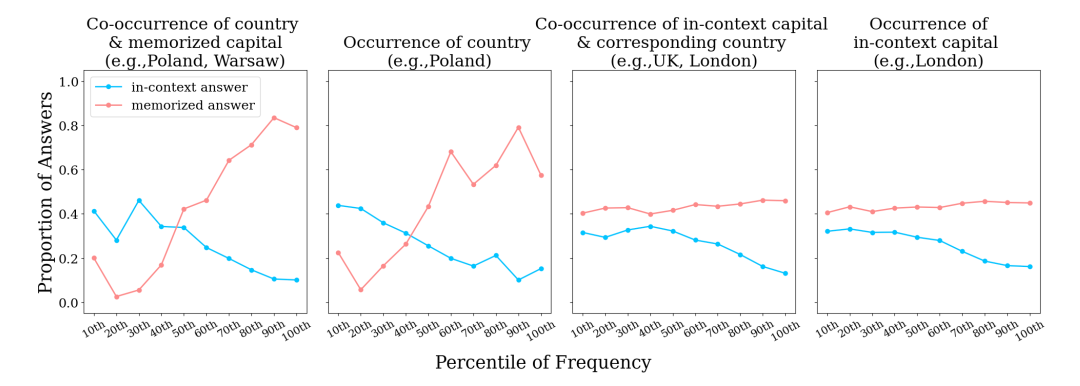
\includegraphics[width=\textwidth]{Mechanisms_plot.png}
	\end{center}
\end{frame}

\begin{frame}{Reading List}
	\begin{large}
		``Language Models are Few-Show Learners''
	\end{large} \\
	Brown et. al

	\quad{}

	\begin{large}
		``Large Language Models Struggle to Learn Long-Tail Knowledge''
	\end{large} \\
	Kandpal et. al

	\quad{}

	\begin{large}
		``What makes in-context learning work?''
	\end{large} \\
	Min et. al
\end{frame}

\section{What's new}
\begin{frame}{New models}
	Currently experimenting with new models. \\
	\begin{itemize}
		\item \textbf{Flan-T5} An encoder-decoder Seq2Seq model.
		\item \textbf{Atlas} Flan T5 fine-tuned with index data.
	\end{itemize}
\end{frame}

\begin{frame}{Technical issues}
	Some technical problem on calculating cross-entropy.

	\vfill{}

	Description of these challenges will be a good part of the written report!
\end{frame}

\section{Hypothesis}
\begin{frame}{Fine-tuning out hypothesis}
	\begin{large}
		\slshape
		Can we predict whether the result from a query with added context came from parametric knowledge, or from the original context? \\[1em]
		Does this change depending on the model? Is there a ``best'' model for preferring contextual knowledge? \\[1em]
		Does this depend on which question is being answered?
	\end{large}

	\vfill{}
	\begin{footnotesize}
		(Work in progress)
	\end{footnotesize}
\end{frame}

\section{Results}

\begin{frame}{More results (now a bit more understandable)}
	\centering
	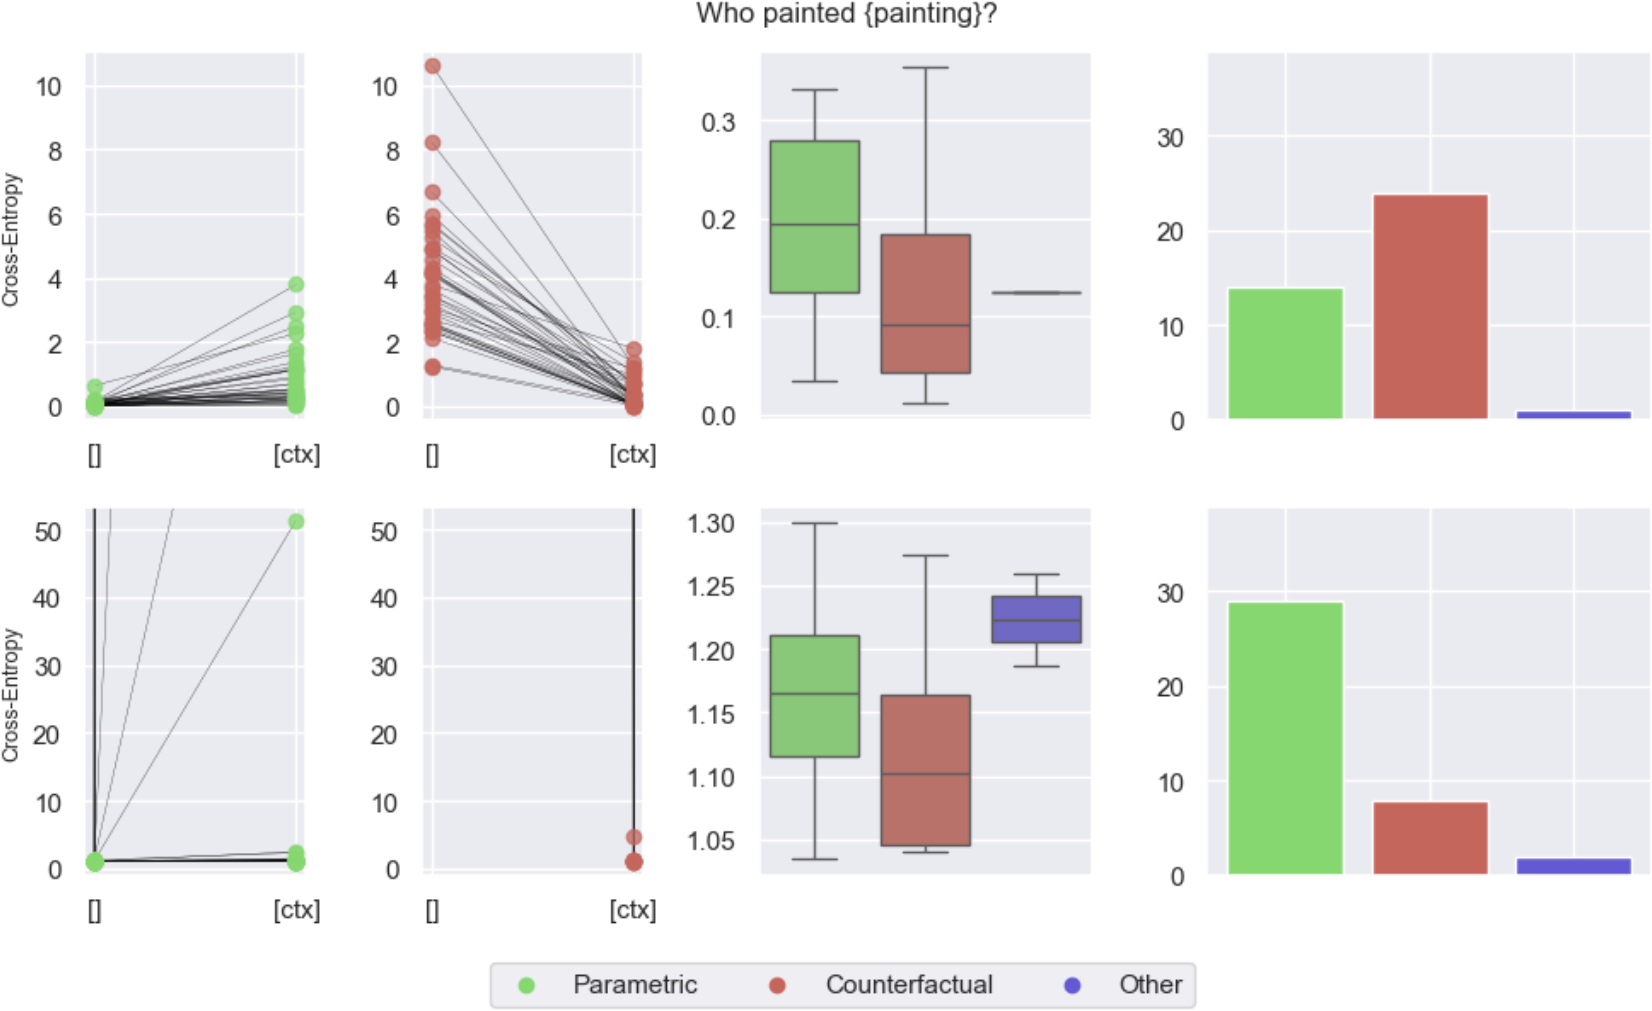
\includegraphics[width=\textwidth]{who_painted_painting.png}
\end{frame}

\begin{frame}{More results (now a bit more understandable)}
	\centering
	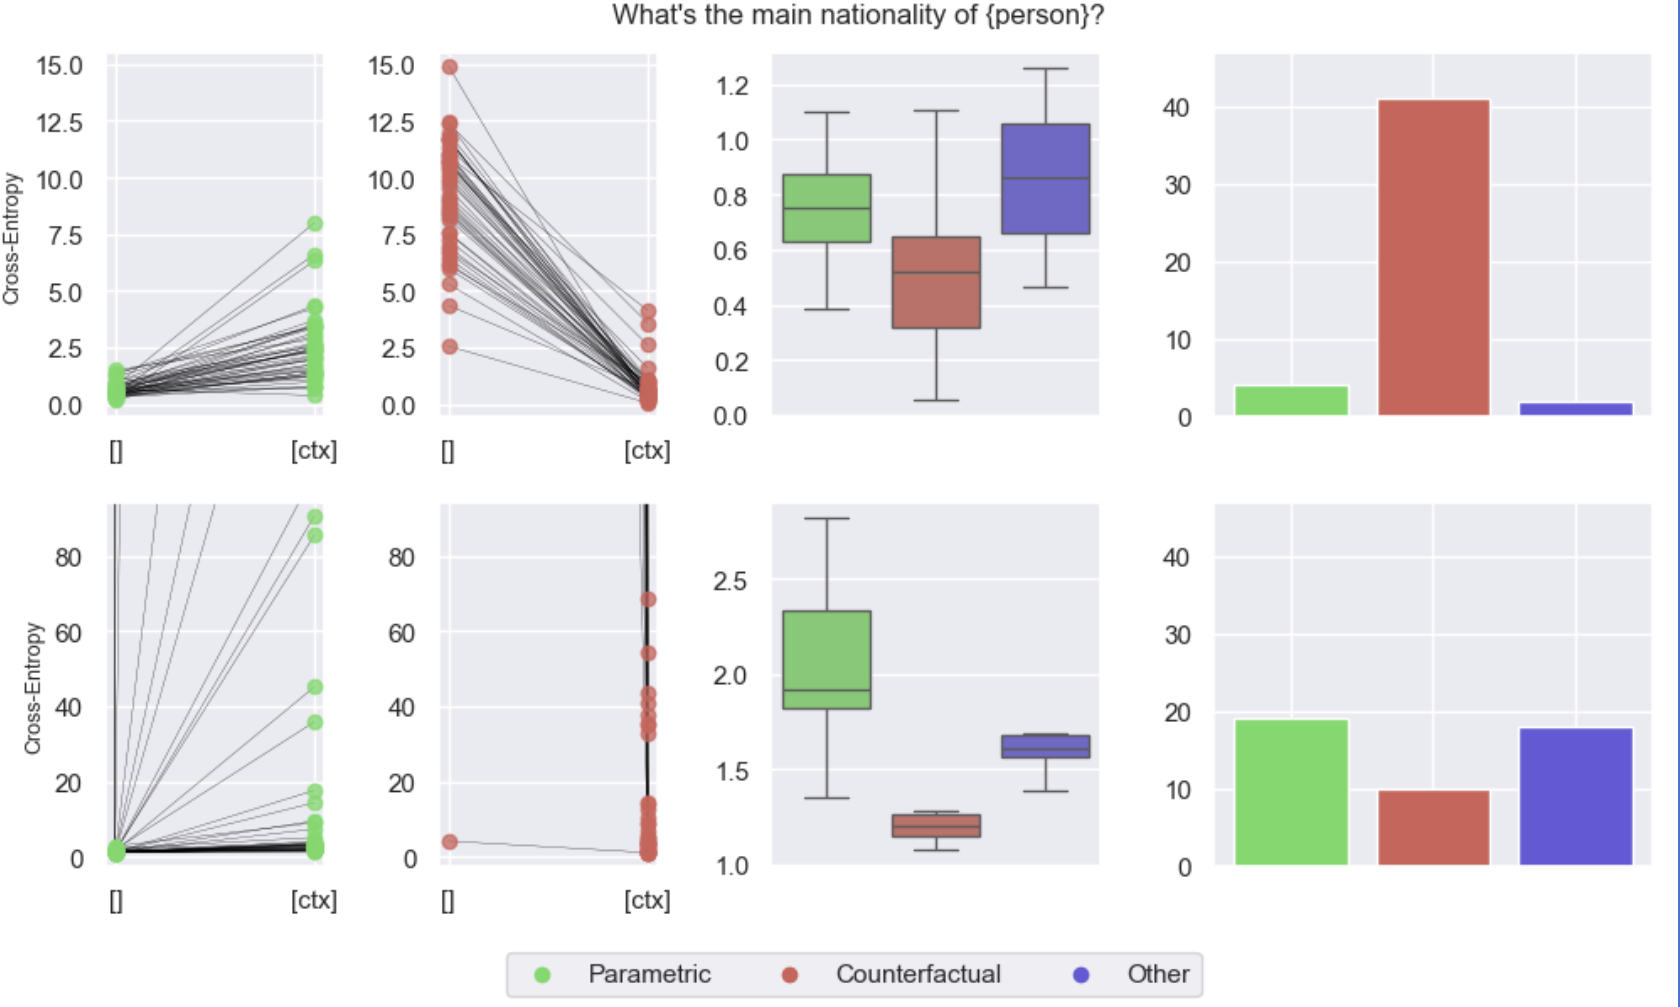
\includegraphics[width=\textwidth]{whats_the_main_nationality_of.png}
\end{frame}

\begin{frame}{More results (now a bit more understandable)}
	\centering
	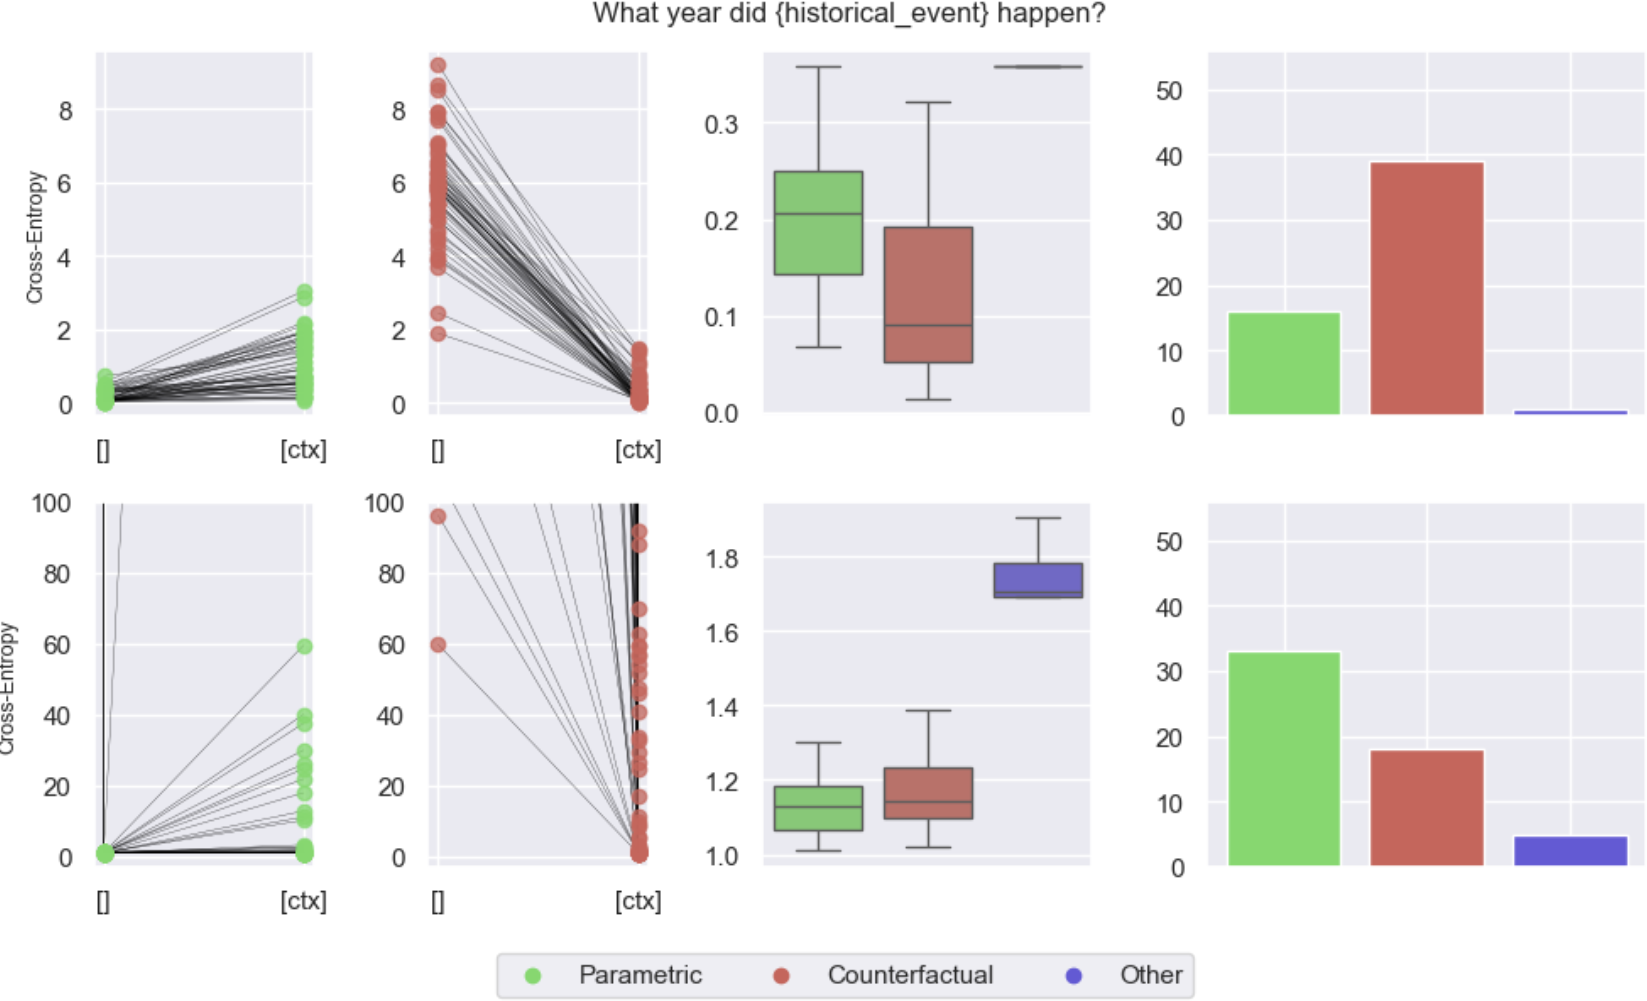
\includegraphics[width=\textwidth]{when_did_event_happen.png}
\end{frame}

\begin{frame}{More results (now a bit more understandable)}
	\centering
	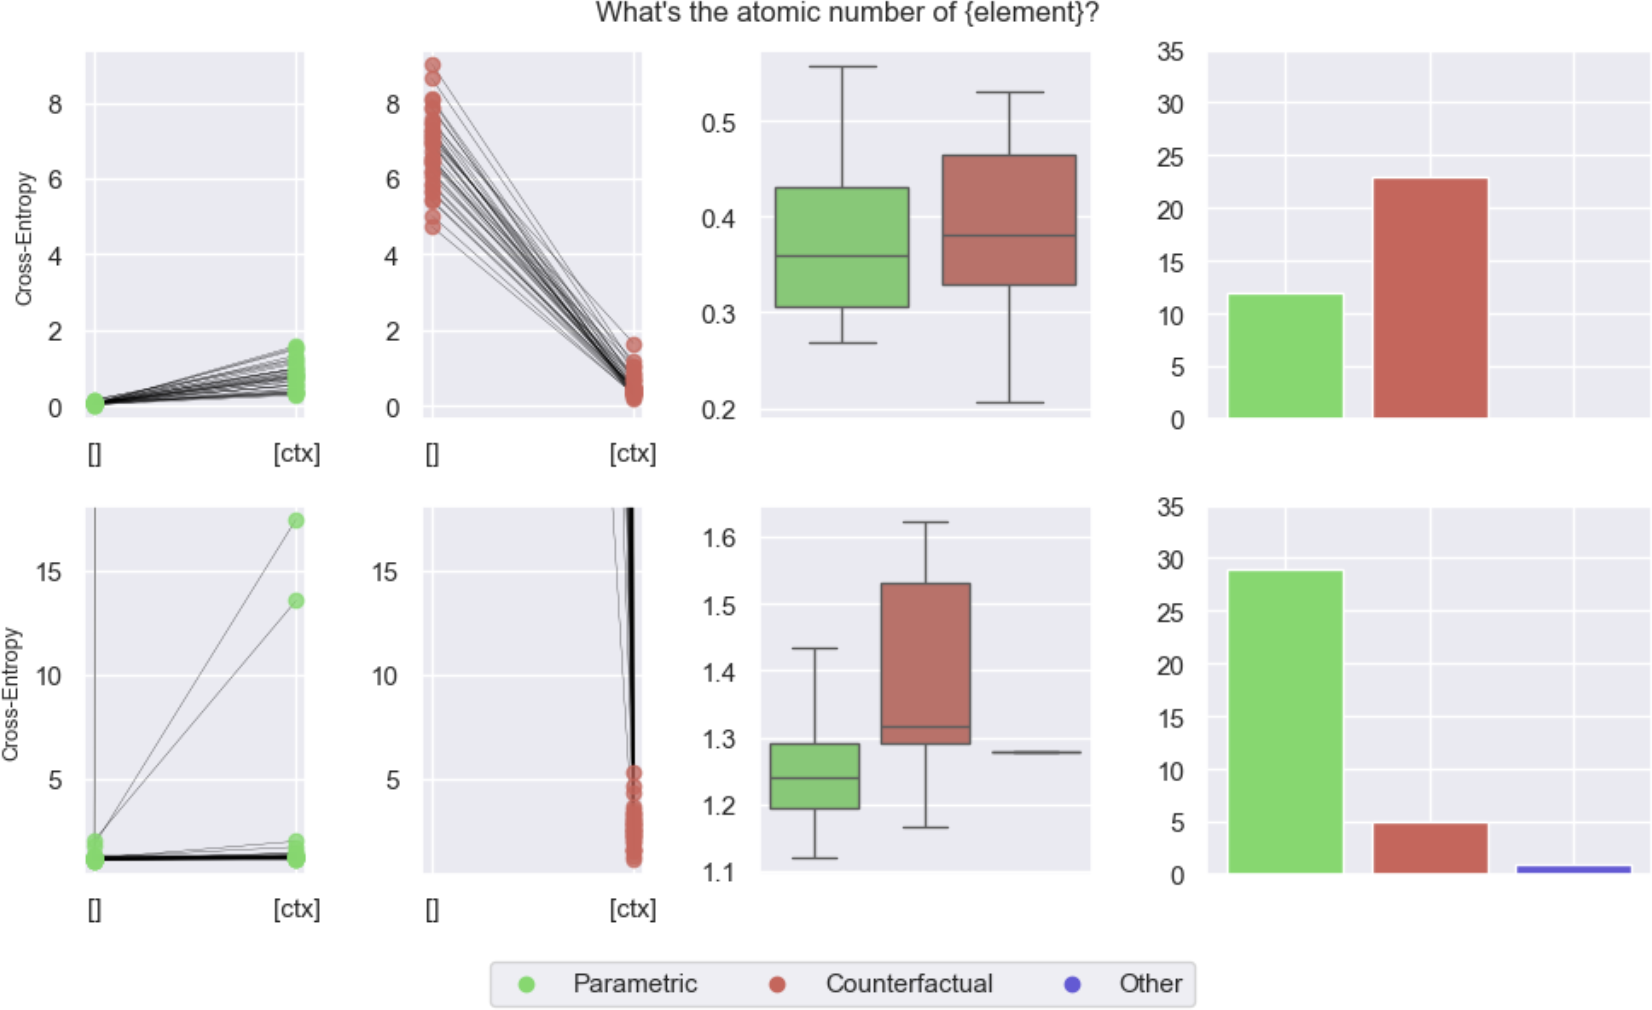
\includegraphics[width=\textwidth]{whats_the_atomic_number_of.png}
\end{frame}

\begin{frame}{Any questions?}
	\begin{Huge}
		\bfseries
		\centering
		Any Questions?
	\end{Huge}
\end{frame}

\end{document}
